% Appendix A

\chapter{Dataset} % Main appendix title

\label{AppendixA} % For referencing this appendix elsewhere, use \ref{AppendixA}

%% dataset a
\begin{figure}[H]
	\centering
	\begin{subfigure}[b]{0.23\linewidth}
		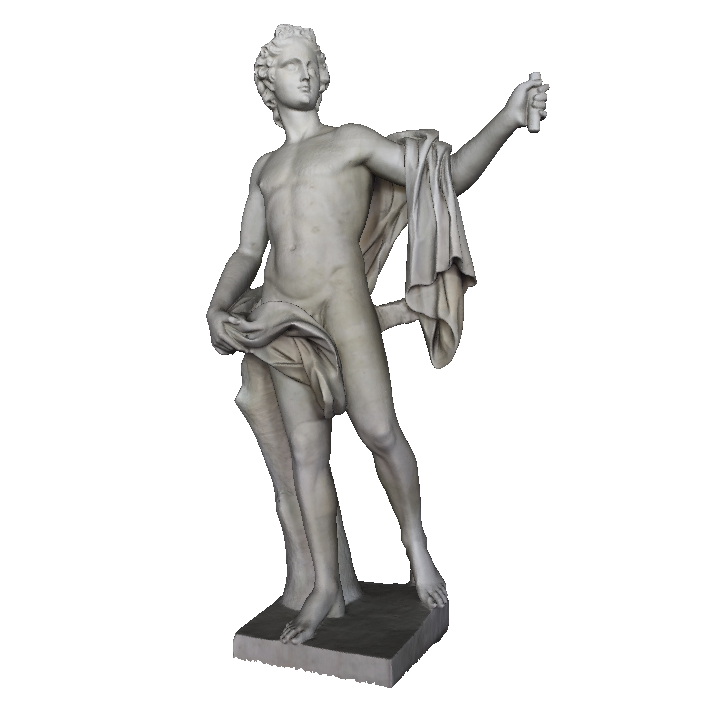
\includegraphics[width=\linewidth]{./Figures/train-dataset/00.apoll.png}
		\caption{apoll}
	\end{subfigure}
	\begin{subfigure}[b]{0.23\linewidth}
		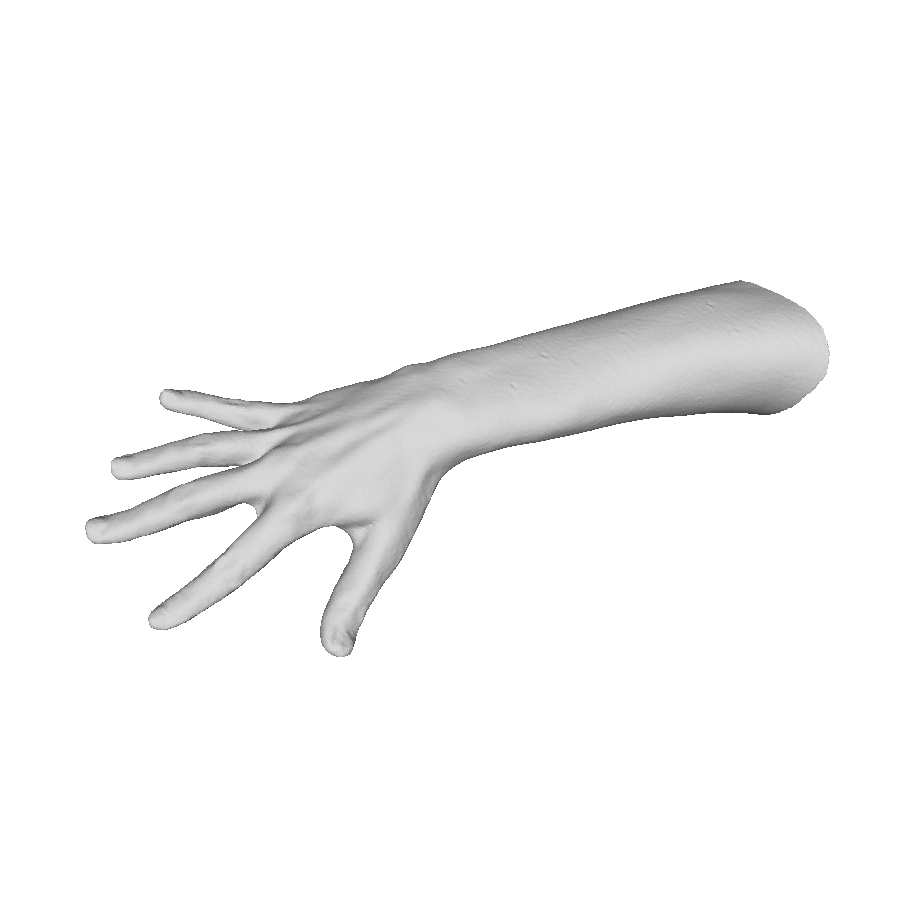
\includegraphics[width=\linewidth]{./Figures/train-dataset/01.arm.png}
		\caption{arm}
	\end{subfigure}
	\begin{subfigure}[b]{0.23\linewidth}
		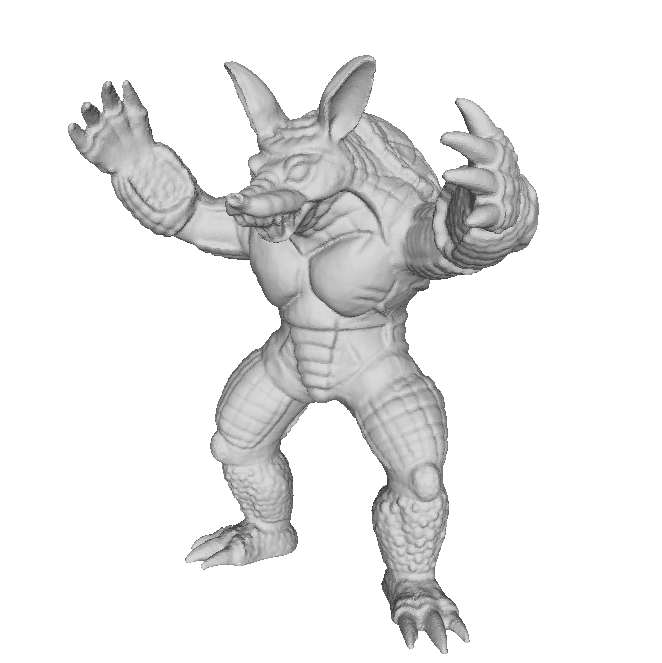
\includegraphics[width=\linewidth]{./Figures/train-dataset/02.armadillo.png}
		\caption{armadillo}
	\end{subfigure}
	\begin{subfigure}[b]{0.23\linewidth}
		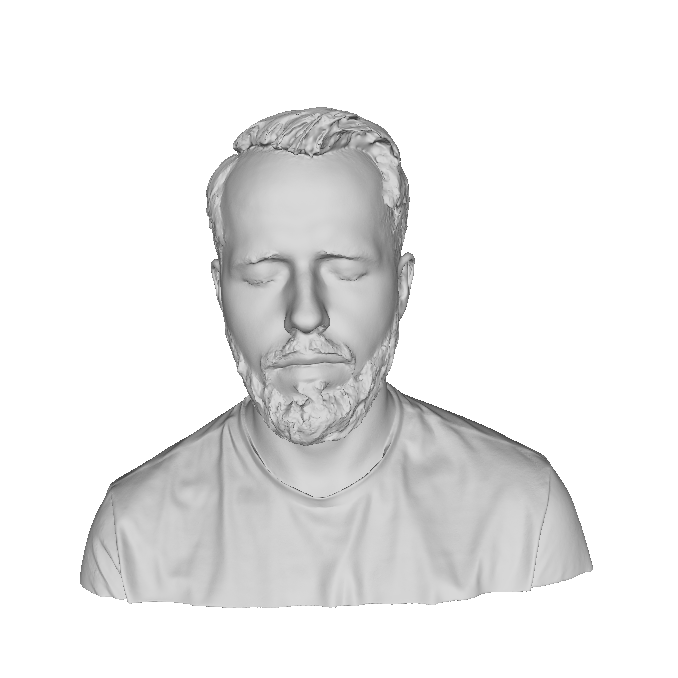
\includegraphics[width=\linewidth]{./Figures/train-dataset/03.bearded-guy.png}
		\caption{bearded-guy}
	\end{subfigure}
	
	\begin{subfigure}[b]{0.23\linewidth}
		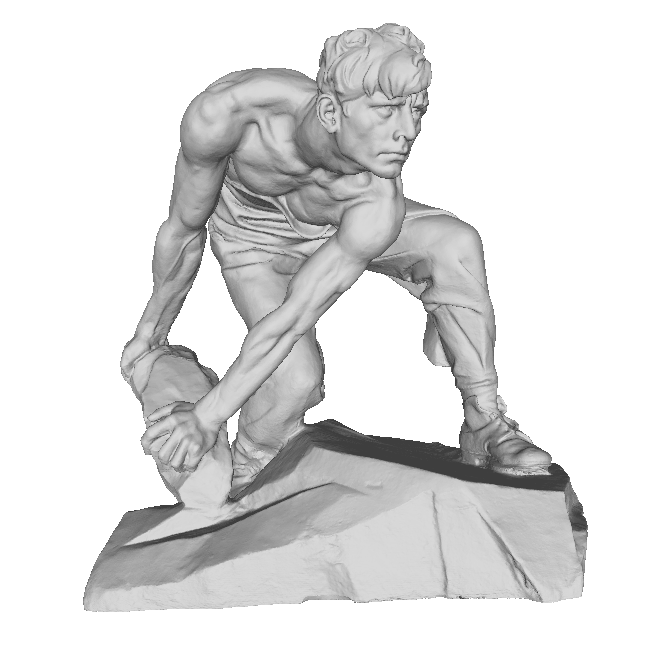
\includegraphics[width=\linewidth]{./Figures/train-dataset/04.bronze-sculpture.png}
		\caption{bronze-sculpture}
	\end{subfigure}
	\begin{subfigure}[b]{0.23\linewidth}
		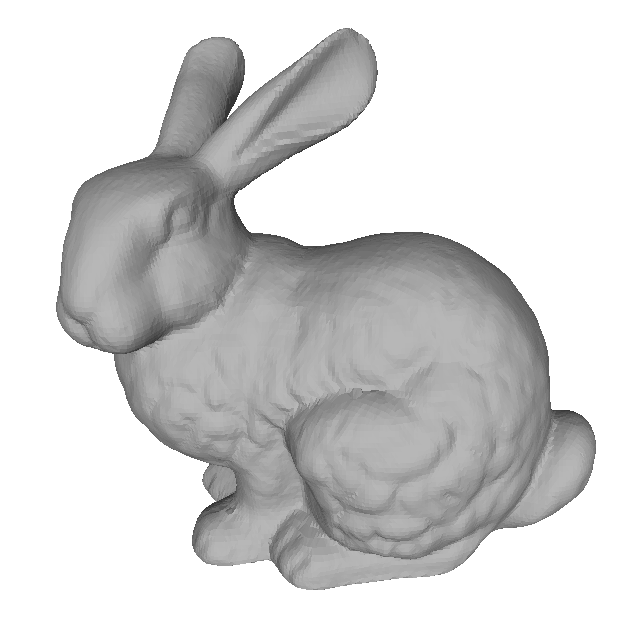
\includegraphics[width=\linewidth]{./Figures/train-dataset/05.bunny.png}
		\caption{bunny}
	\end{subfigure}
	\begin{subfigure}[b]{0.23\linewidth}
		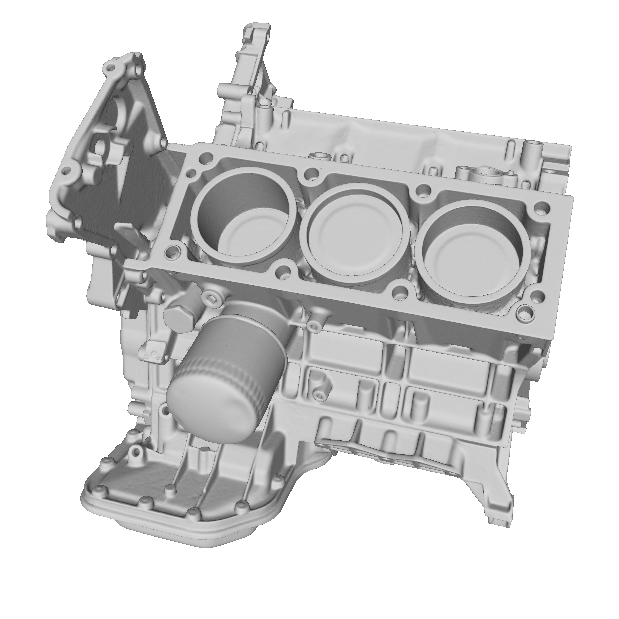
\includegraphics[width=\linewidth]{./Figures/train-dataset/06.car-engine.png}
		\caption{car-engine}
	\end{subfigure}
	\begin{subfigure}[b]{0.23\linewidth}
		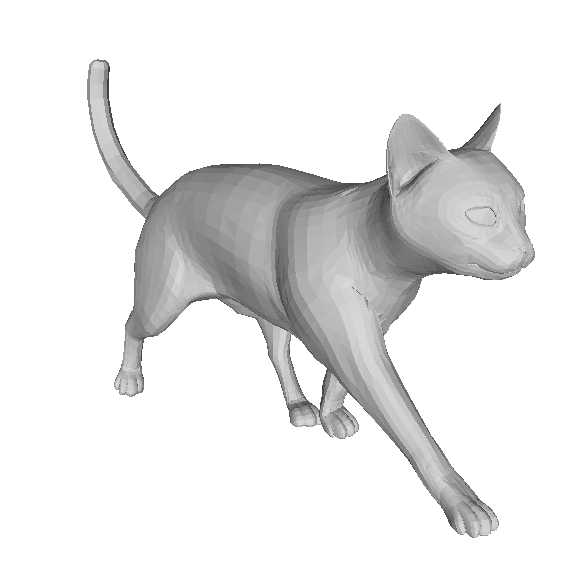
\includegraphics[width=\linewidth]{./Figures/train-dataset/07.cat.png}
		\caption{cat}
	\end{subfigure}
	
	\begin{subfigure}[b]{0.23\linewidth}
		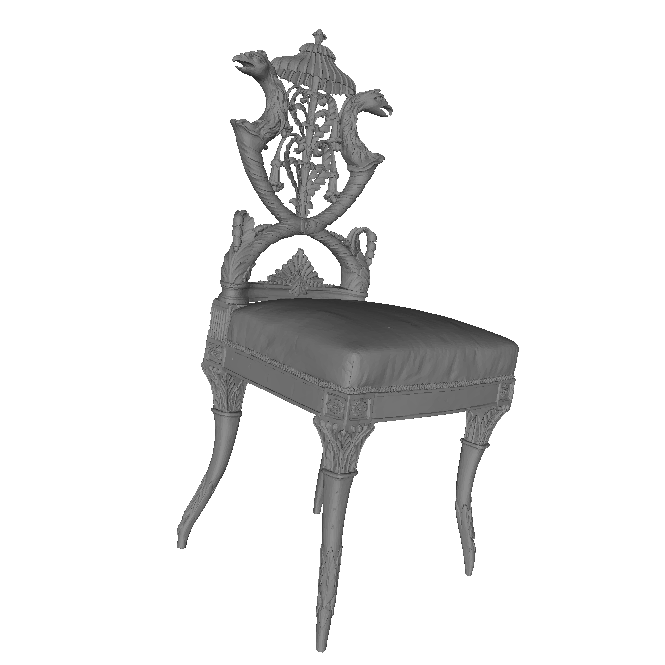
\includegraphics[width=\linewidth]{./Figures/train-dataset/08.pergolesi-side-chair.png}
		\caption{side-chair}
	\end{subfigure}
	\begin{subfigure}[b]{0.23\linewidth}
		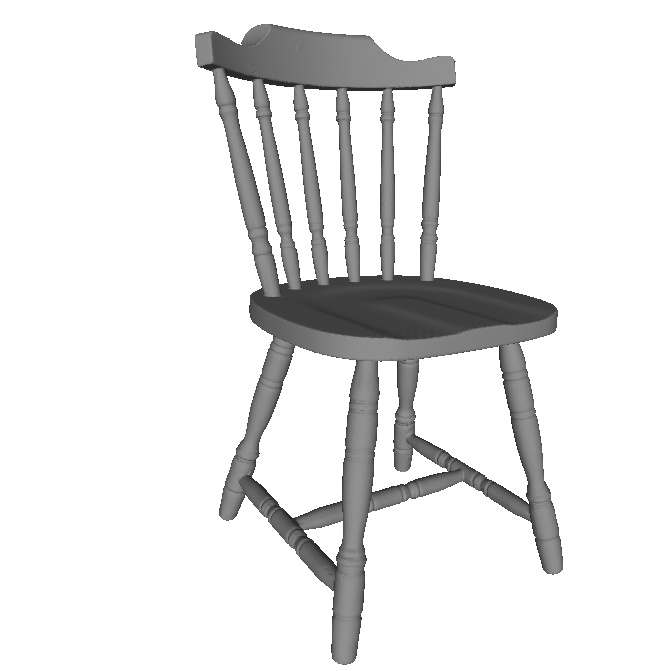
\includegraphics[width=\linewidth]{./Figures/train-dataset/09.chair2.png}
		\caption{chair2}
	\end{subfigure}
	\begin{subfigure}[b]{0.23\linewidth}
		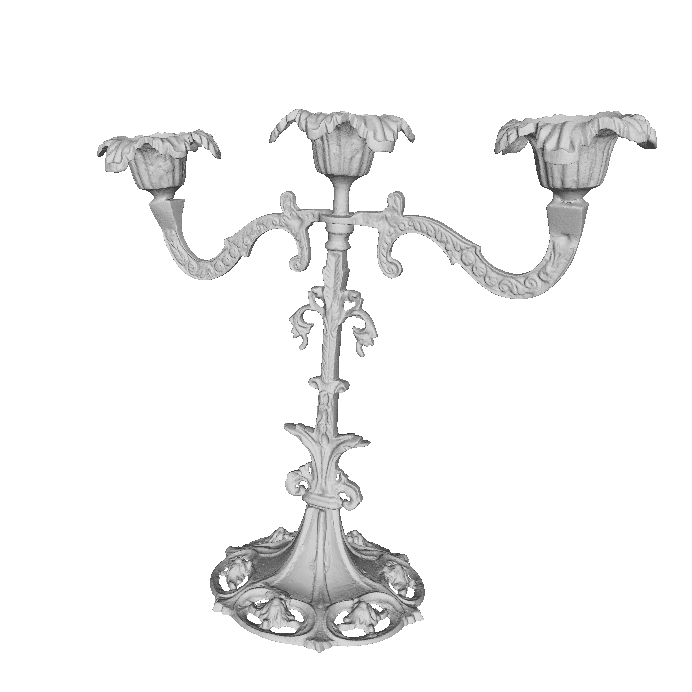
\includegraphics[width=\linewidth]{./Figures/train-dataset/10.chandelier.png}
		\caption{chandelier}
	\end{subfigure}
	\begin{subfigure}[b]{0.23\linewidth}
		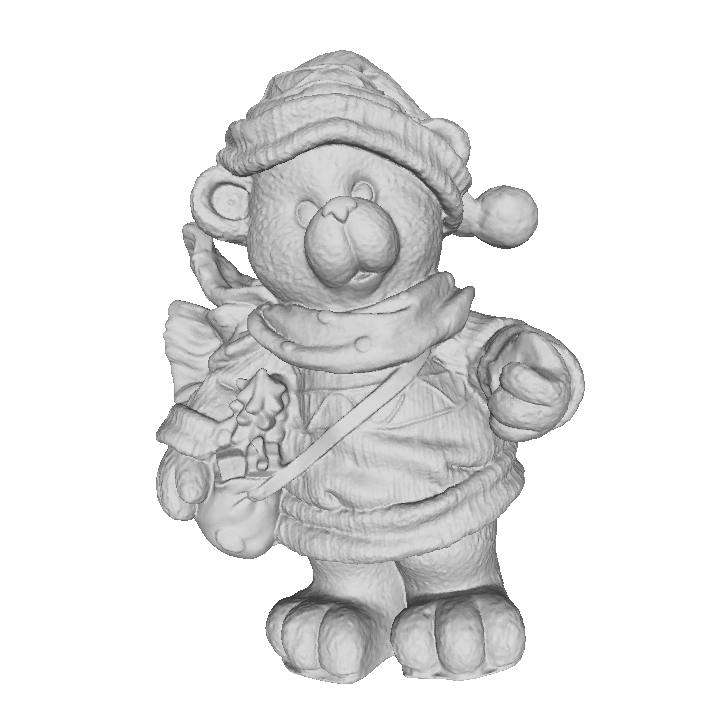
\includegraphics[width=\linewidth]{./Figures/train-dataset/11.christmas-bear.png}
		\caption{Christmas-bear}
	\end{subfigure}

	\begin{subfigure}[b]{0.23\linewidth}
		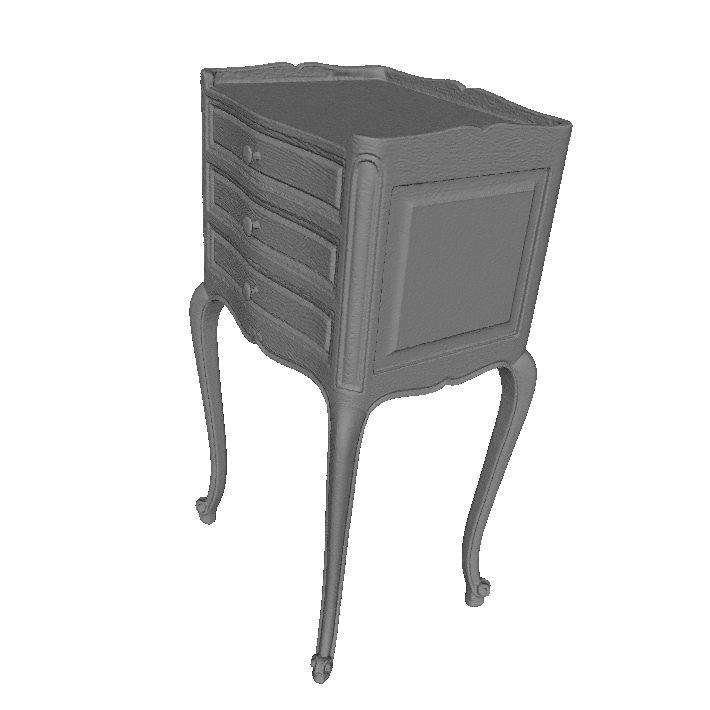
\includegraphics[width=\linewidth]{./Figures/train-dataset/12.classic-side-table.png}
		\caption{classic-side-table}
	\end{subfigure}
	\begin{subfigure}[b]{0.23\linewidth}
		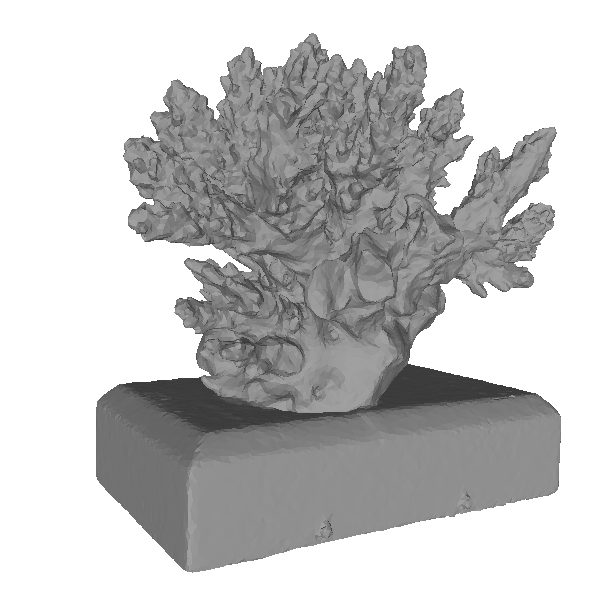
\includegraphics[width=\linewidth]{./Figures/train-dataset/13.coral.png}
		\caption{coral}
	\end{subfigure}
	\begin{subfigure}[b]{0.23\linewidth}
		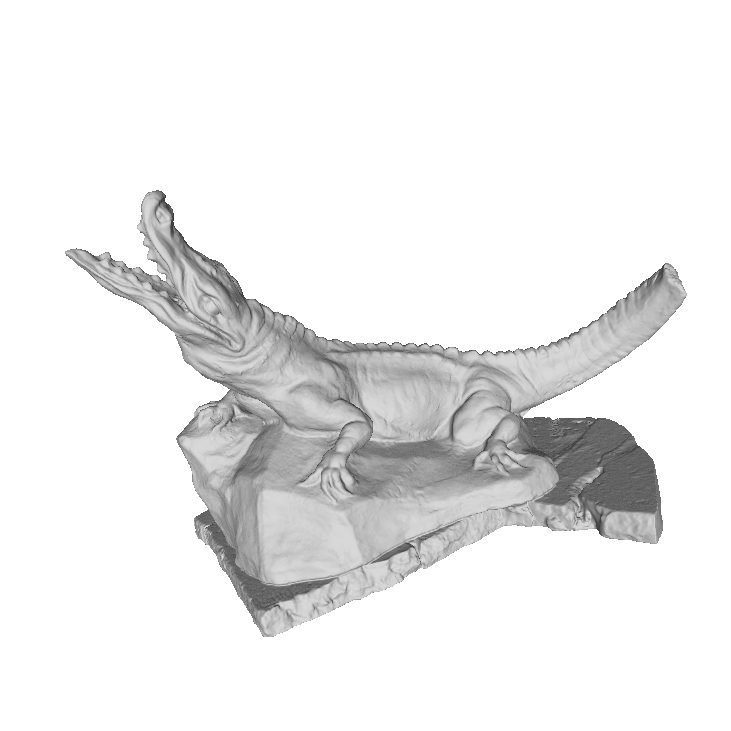
\includegraphics[width=\linewidth]{./Figures/train-dataset/14.crocodile-statue.png}
		\caption{crocodile-statue}
	\end{subfigure}
	\begin{subfigure}[b]{0.23\linewidth}
		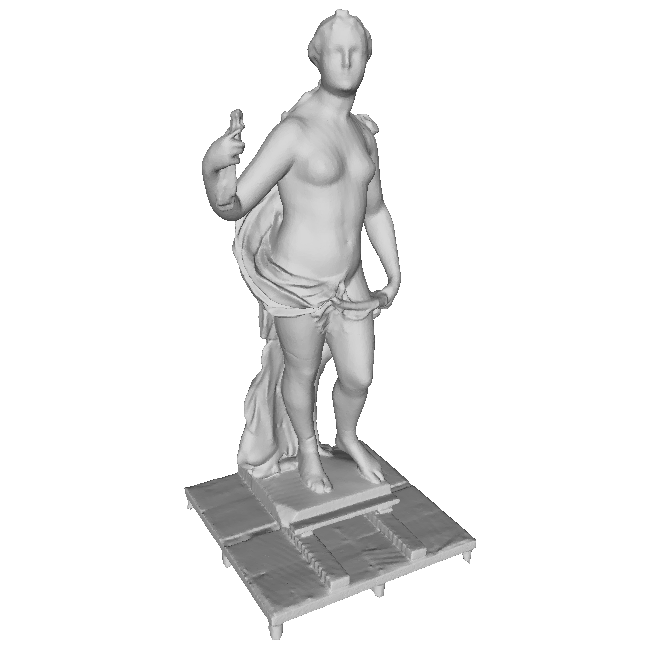
\includegraphics[width=\linewidth]{./Figures/train-dataset/15.diane.png}
		\caption{Diane}
	\end{subfigure}

	\label{fig:dataset_a}
\caption{Point clouds in training dataset A }
\end{figure}


%% dataset b 
\begin{figure}
	\centering
	\begin{subfigure}[b]{0.23\linewidth}
		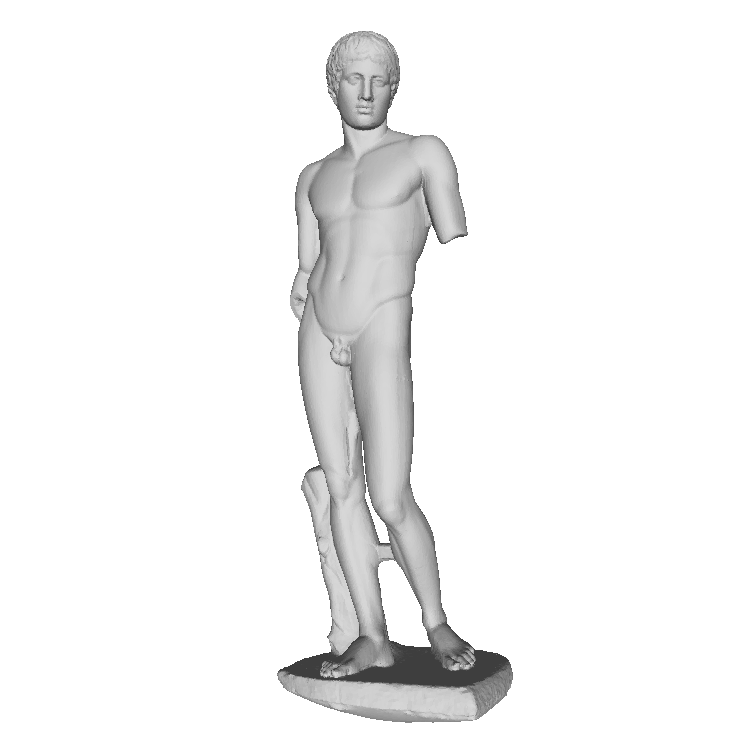
\includegraphics[width=\linewidth]{./Figures/train-dataset/16.dresdner-knabe.png}
		\caption{Dresdner-knabe}
	\end{subfigure}
	\begin{subfigure}[b]{0.23\linewidth}
		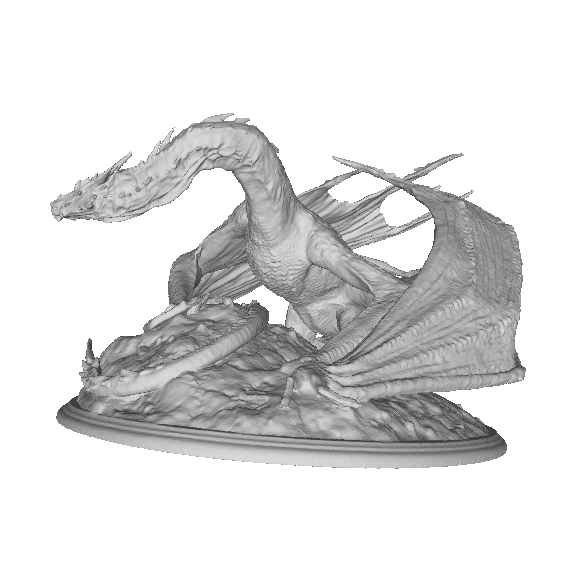
\includegraphics[width=\linewidth]{./Figures/train-dataset/17.fantasy-dragon.png}
		\caption{fantasy-dragon}
	\end{subfigure}
	\begin{subfigure}[b]{0.23\linewidth}
		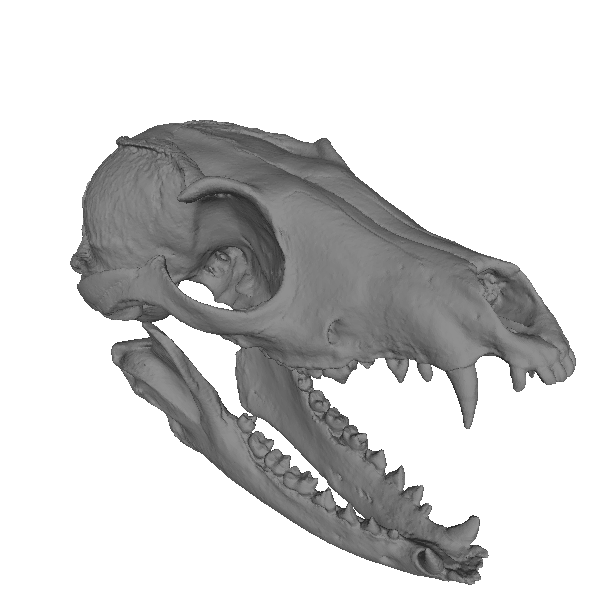
\includegraphics[width=\linewidth]{./Figures/train-dataset/18.fox-skull.png}
		\caption{fox-skull}
	\end{subfigure}
	\begin{subfigure}[b]{0.23\linewidth}
		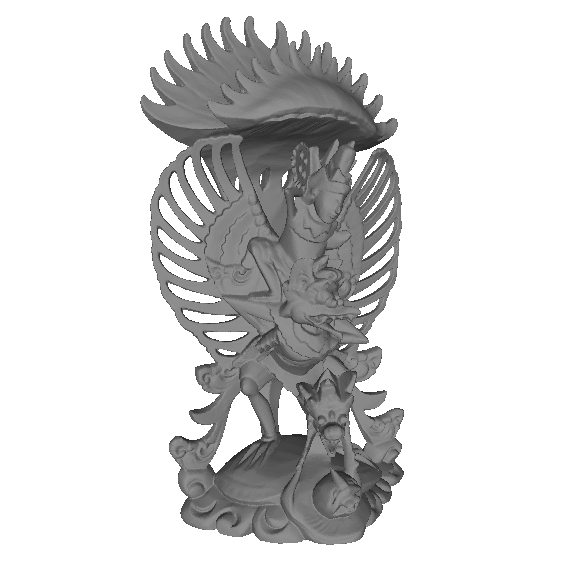
\includegraphics[width=\linewidth]{./Figures/train-dataset/19.garuda-and-vishnu.png}
		\caption{Garuda and Vishnu}
	\end{subfigure}
	
	\begin{subfigure}[b]{0.23\linewidth}
		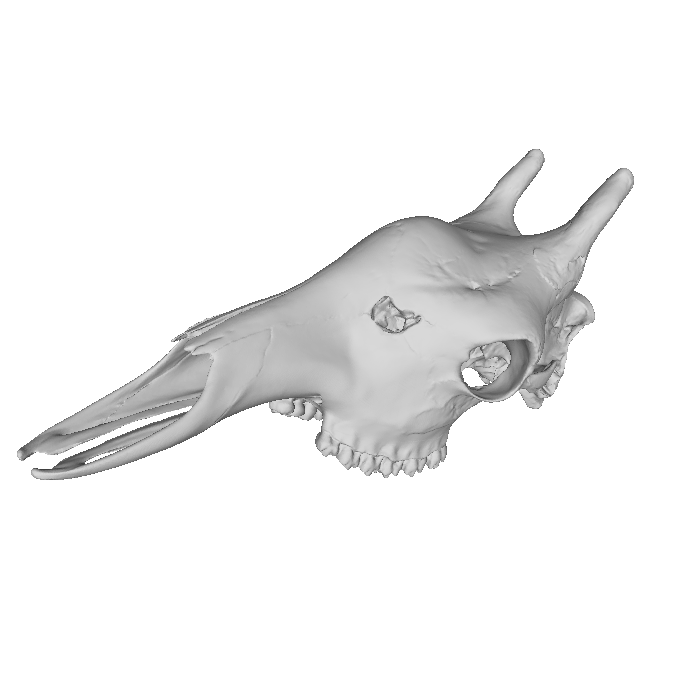
\includegraphics[width=\linewidth]{./Figures/train-dataset/20.giraffe-skull.png}
		\caption{giraffe-skull}
	\end{subfigure}
	\begin{subfigure}[b]{0.23\linewidth}
		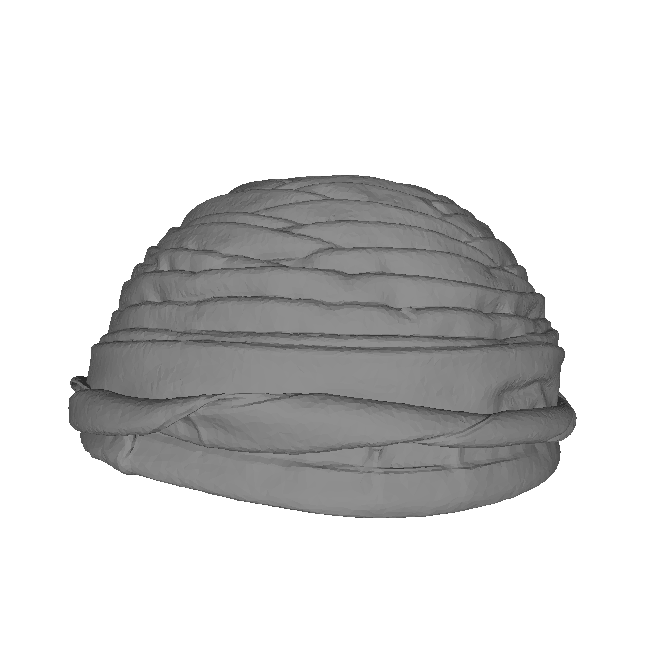
\includegraphics[width=\linewidth]{./Figures/train-dataset/21.green-hat.png}
		\caption{green-hat}
	\end{subfigure}
	\begin{subfigure}[b]{0.23\linewidth}
		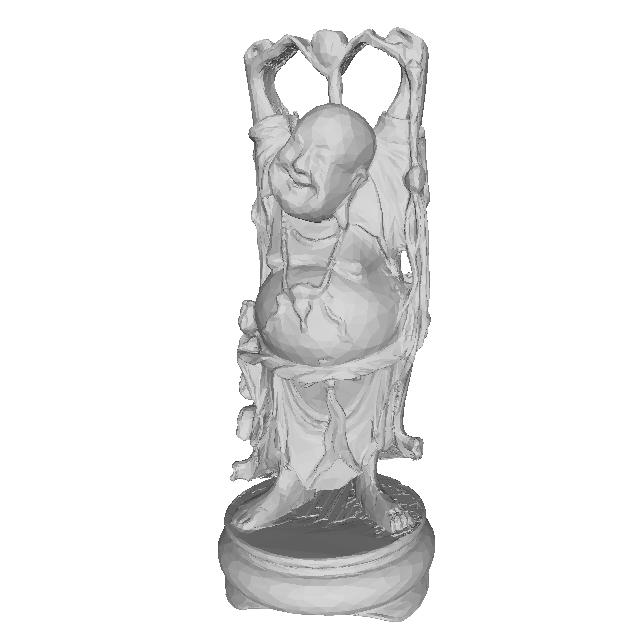
\includegraphics[width=\linewidth]{./Figures/train-dataset/22.happy-buddha.png}
		\caption{happy-budda}
	\end{subfigure}
	\begin{subfigure}[b]{0.23\linewidth}
		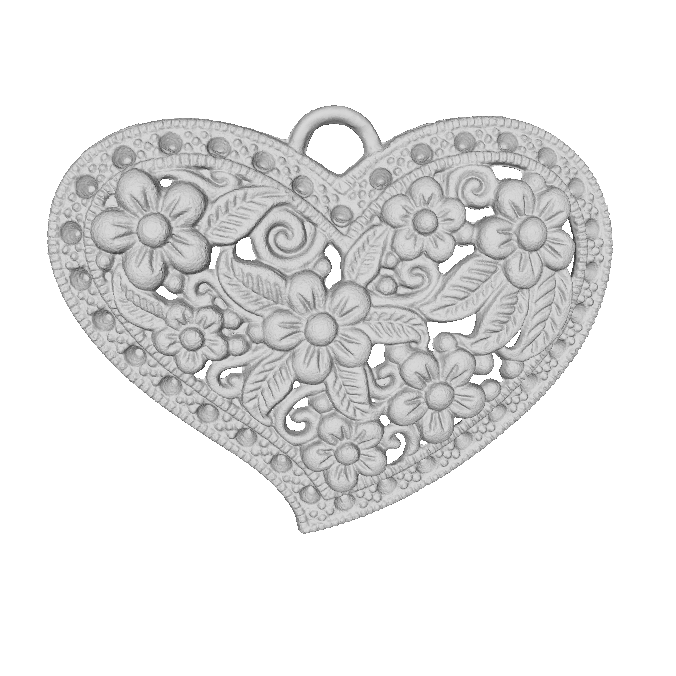
\includegraphics[width=\linewidth]{./Figures/train-dataset/23.heart-pendant.png}
		\caption{heart-pendant}
	\end{subfigure}
	
		\begin{subfigure}[b]{0.23\linewidth}
		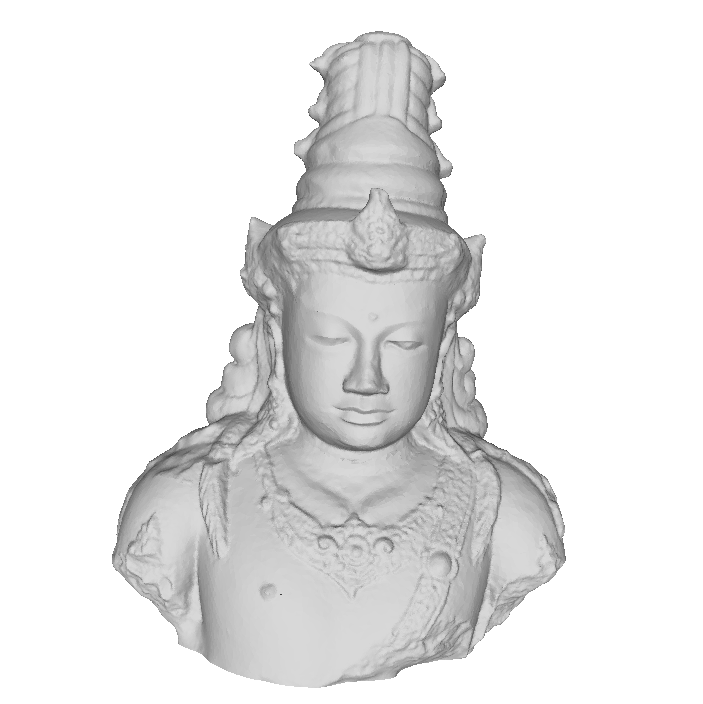
\includegraphics[width=\linewidth]{./Figures/train-dataset/24.indonesian-statue.png}
		\caption{indonesian-statue}
	\end{subfigure}
	\begin{subfigure}[b]{0.23\linewidth}
		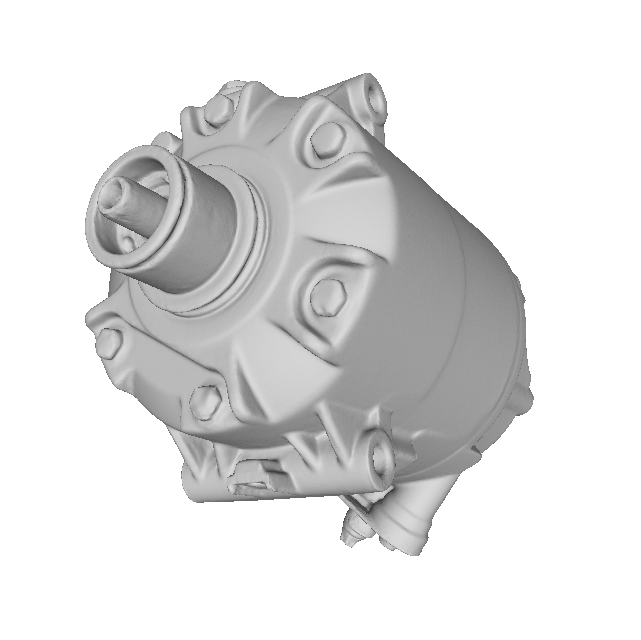
\includegraphics[width=\linewidth]{./Figures/train-dataset/25.industrial-compressor.png}
		\caption{industrial-compressor}
	\end{subfigure}
	\begin{subfigure}[b]{0.23\linewidth}
		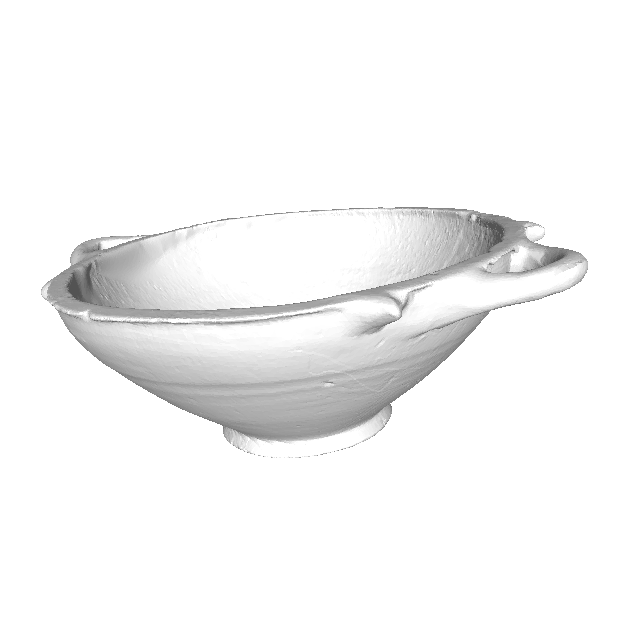
\includegraphics[width=\linewidth]{./Figures/train-dataset/26.kylix.png}
		\caption{kylix}
	\end{subfigure}
	\begin{subfigure}[b]{0.23\linewidth}
		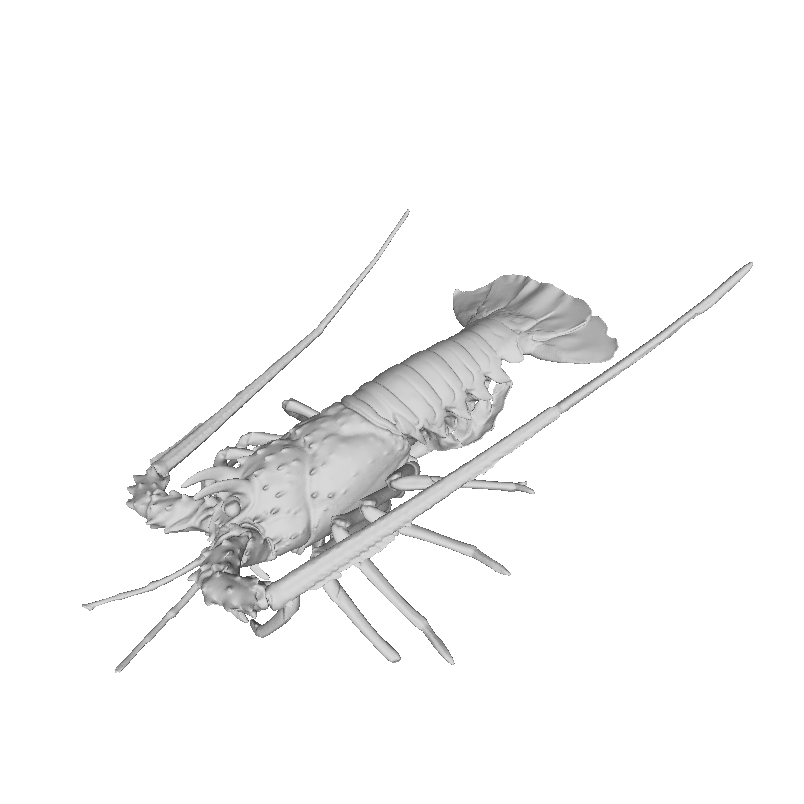
\includegraphics[width=\linewidth]{./Figures/train-dataset/27.lobster.png}
		\caption{lobster}
	\end{subfigure}
	
	\begin{subfigure}[b]{0.23\linewidth}
		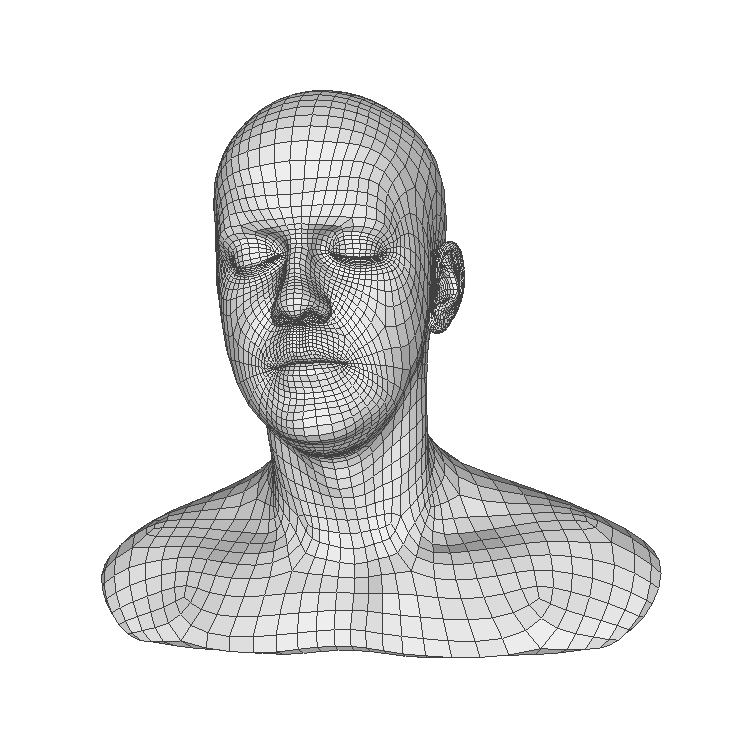
\includegraphics[width=\linewidth]{./Figures/train-dataset/28.head.png}
		\caption{head}
	\end{subfigure}
	\begin{subfigure}[b]{0.23\linewidth}
		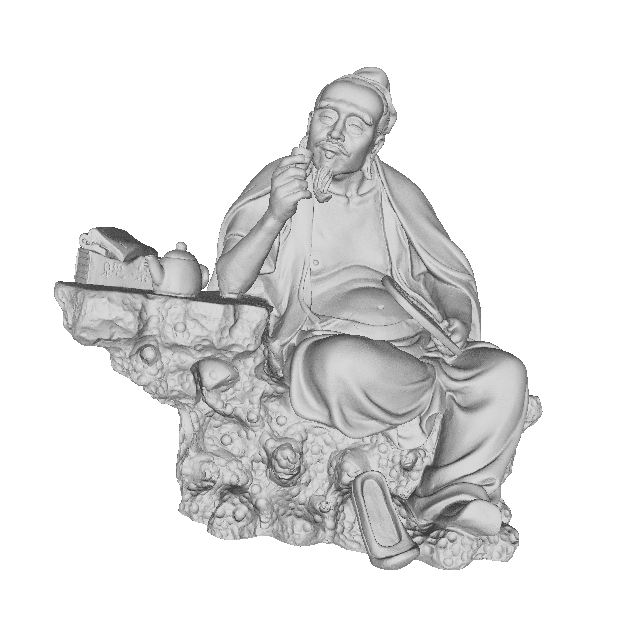
\includegraphics[width=\linewidth]{./Figures/train-dataset/29.Lu-Yu.png}
		\caption{Lu-Yu}
	\end{subfigure}
	\begin{subfigure}[b]{0.23\linewidth}
		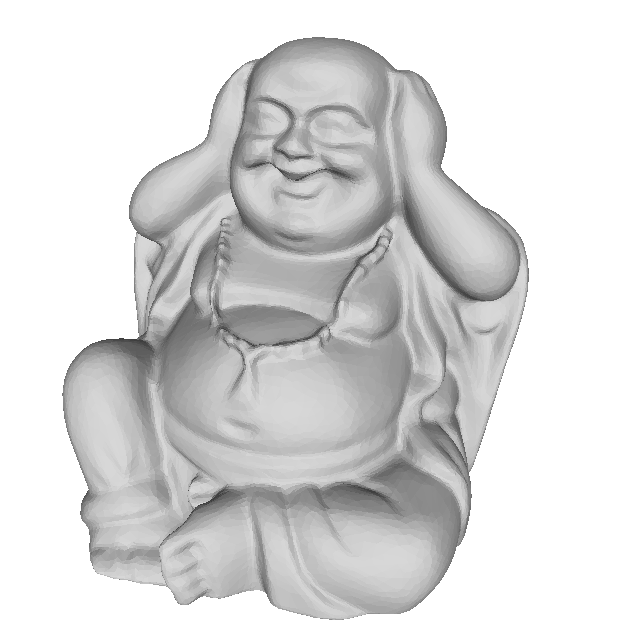
\includegraphics[width=\linewidth]{./Figures/train-dataset/30.maitreya.png}
		\caption{Maitreya}
	\end{subfigure}
	\begin{subfigure}[b]{0.23\linewidth}
		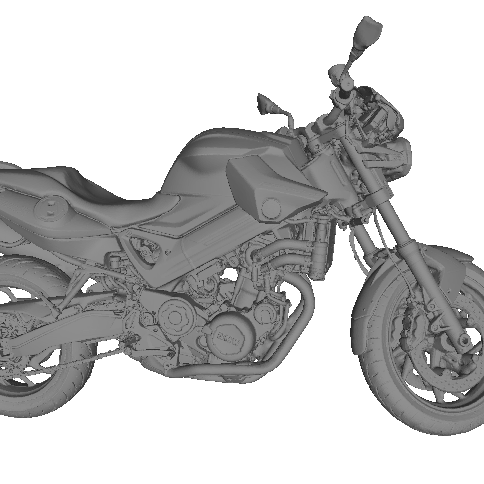
\includegraphics[width=\linewidth]{./Figures/train-dataset/31.motorbike.png}
		\caption{motorbike}
	\end{subfigure}
	
	
	\begin{subfigure}[b]{0.23\linewidth}
		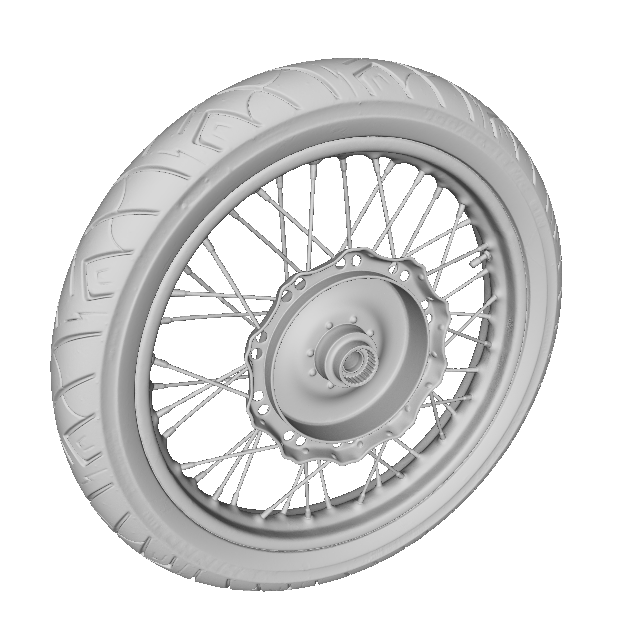
\includegraphics[width=\linewidth]{./Figures/train-dataset/32.motorcycle-wheel.png}
		\caption{motorcycle-wheel}
	\end{subfigure}
	\begin{subfigure}[b]{0.23\linewidth}
		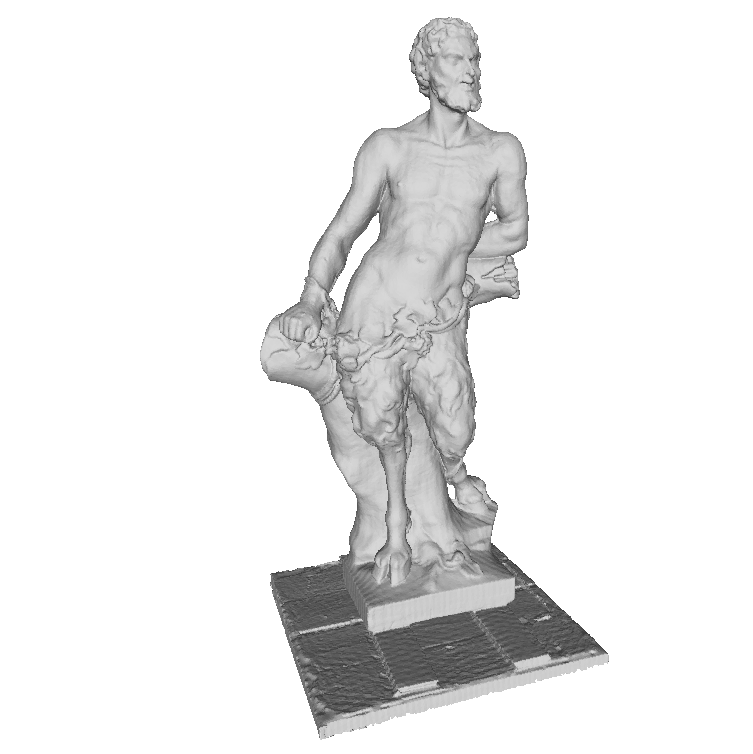
\includegraphics[width=\linewidth]{./Figures/train-dataset/33.pan.png}
		\caption{Pan}
	\end{subfigure}
	\begin{subfigure}[b]{0.23\linewidth}
		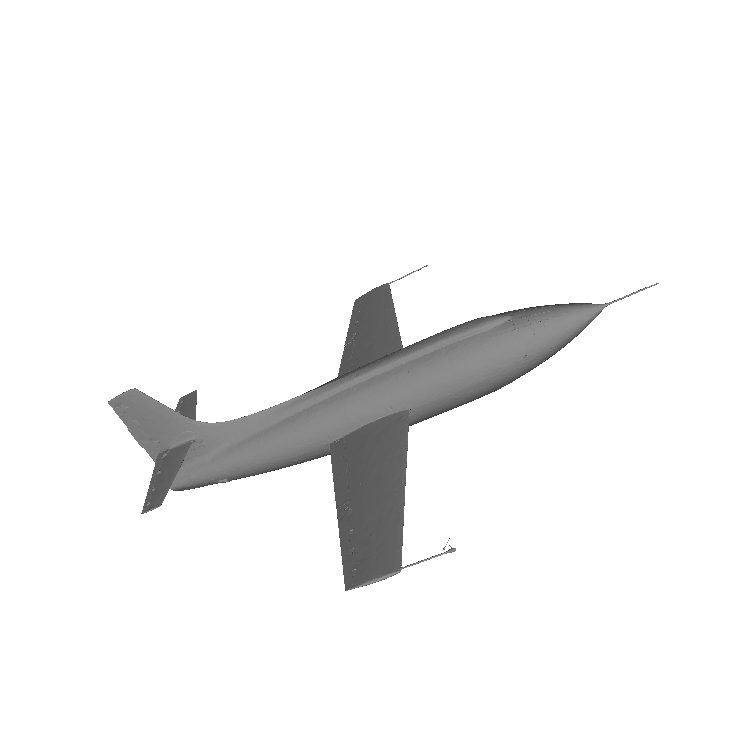
\includegraphics[width=\linewidth]{./Figures/train-dataset/34.plane.png}
		\caption{plane}
	\end{subfigure}
	\begin{subfigure}[b]{0.23\linewidth}
		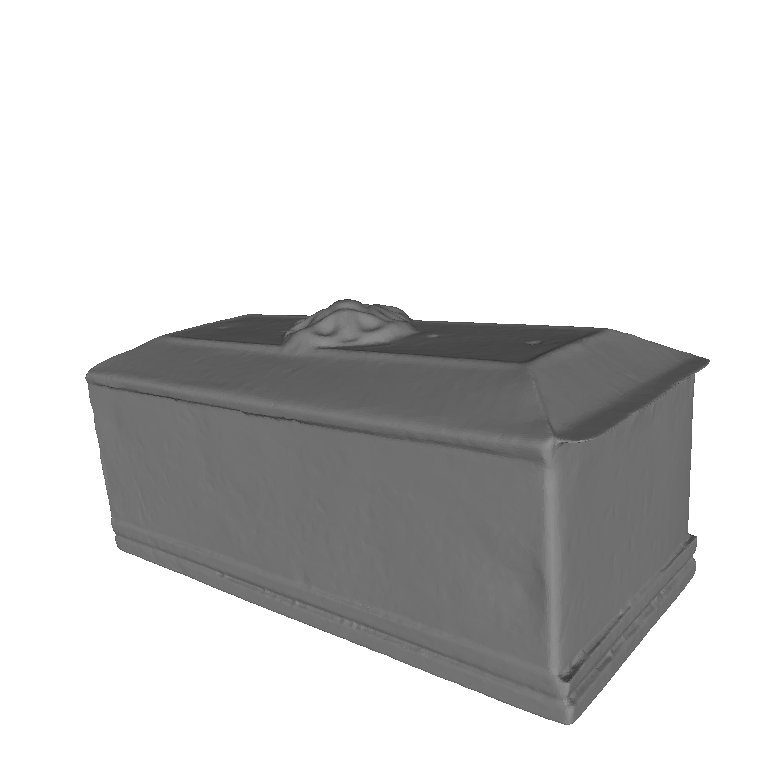
\includegraphics[width=\linewidth]{./Figures/train-dataset/35.elkins-refrigerator.png}
		\caption{elkins-refrigerator}
	\end{subfigure}
	

	
	
	\label{fig:dataset_b}
	\caption{Point clouds in training dataset B }
\end{figure}



%% dataset c 
\begin{figure}
	\centering

	\begin{subfigure}[b]{0.23\linewidth}
	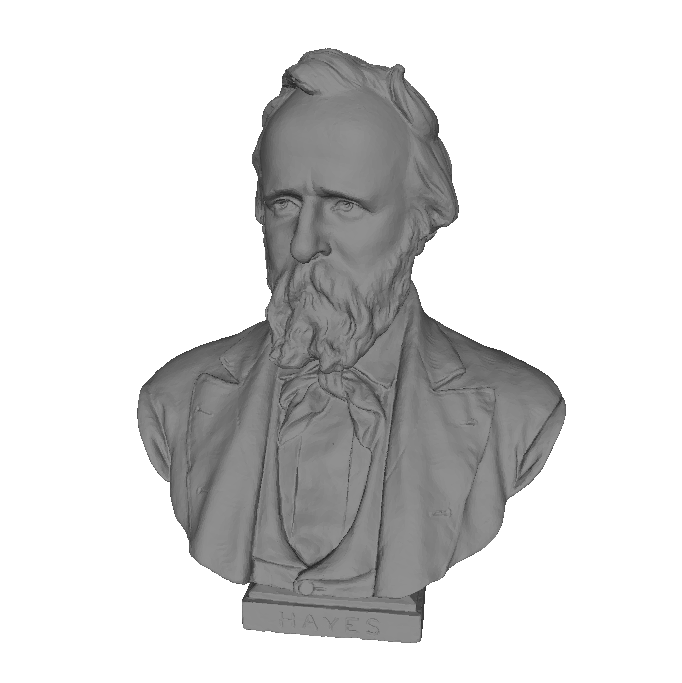
\includegraphics[width=\linewidth]{./Figures/train-dataset/36.rutherford-b-hayes-plaster.png}
	\caption{Rutherford}
\end{subfigure}
\begin{subfigure}[b]{0.23\linewidth}
	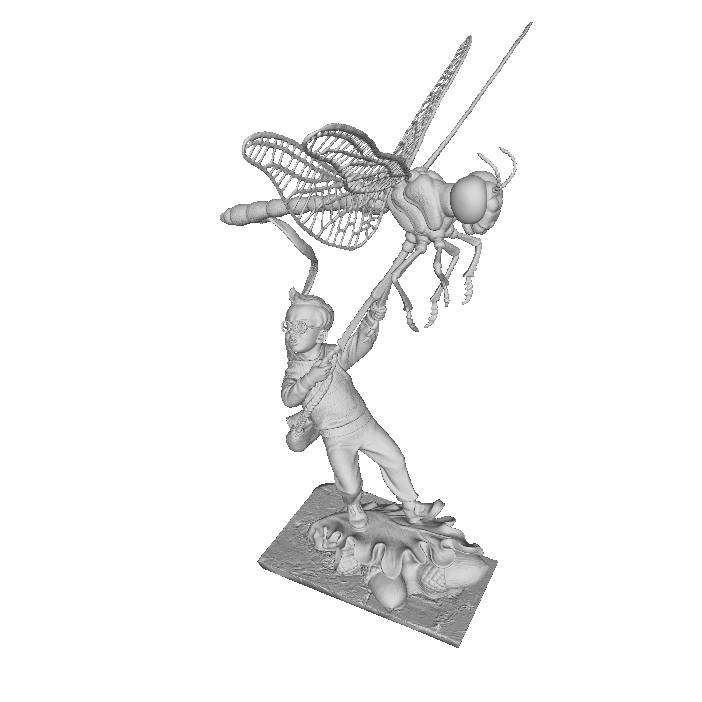
\includegraphics[width=\linewidth]{./Figures/train-dataset/37.statue-dragonfly-tamer.png}
	\caption{statue-dragonfly-tamer}
\end{subfigure}
\begin{subfigure}[b]{0.23\linewidth}
	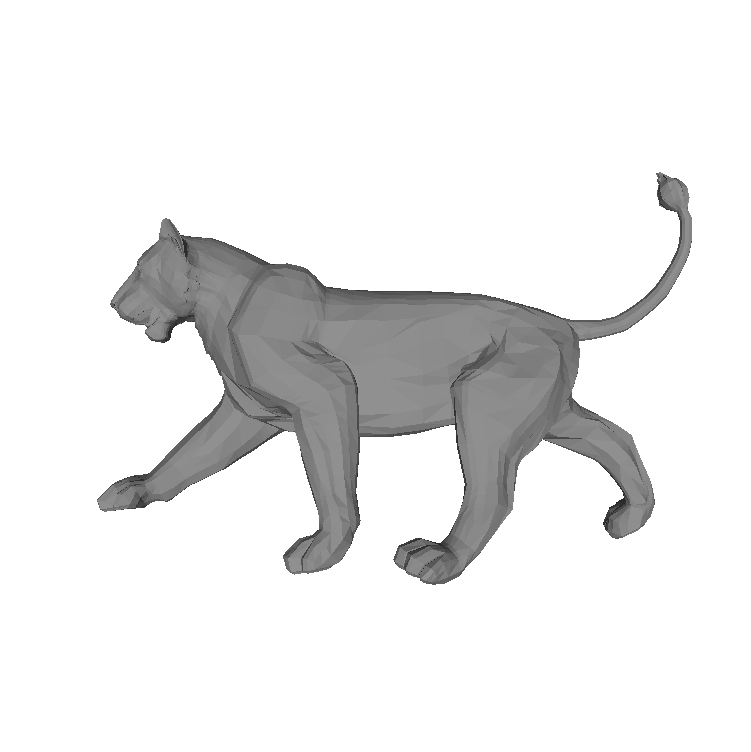
\includegraphics[width=\linewidth]{./Figures/train-dataset/38.tiger.png}
	\caption{Tiger}
\end{subfigure}
\begin{subfigure}[b]{0.23\linewidth}
	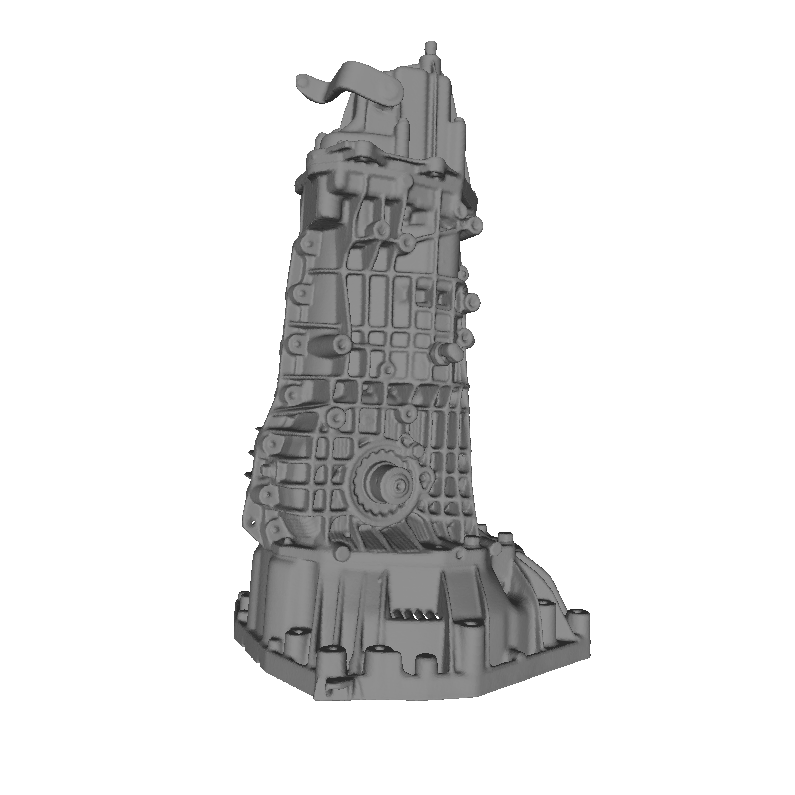
\includegraphics[width=\linewidth]{./Figures/train-dataset/39.transmission.png}
	\caption{transmission}
\end{subfigure}

	\begin{subfigure}[b]{0.23\linewidth}
		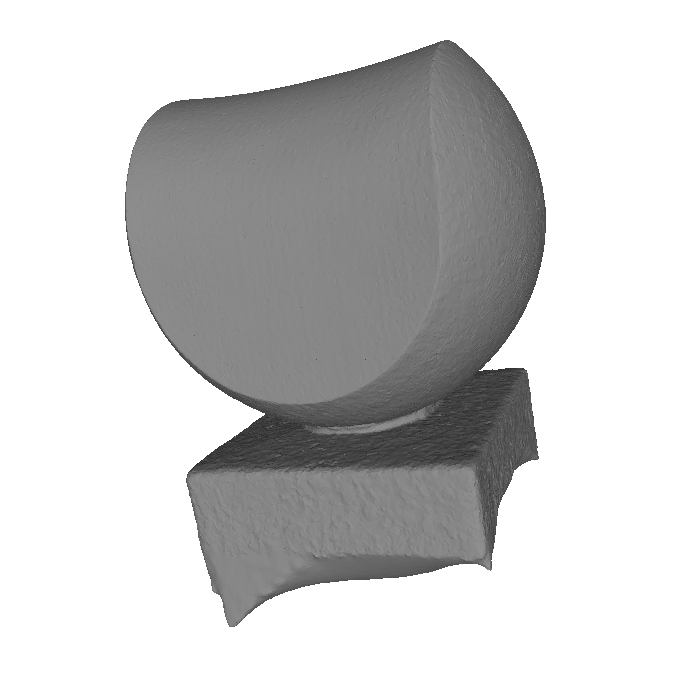
\includegraphics[width=\linewidth]{./Figures/train-dataset/40.universe.png}
		\caption{universe}
	\end{subfigure}
	\begin{subfigure}[b]{0.23\linewidth}
		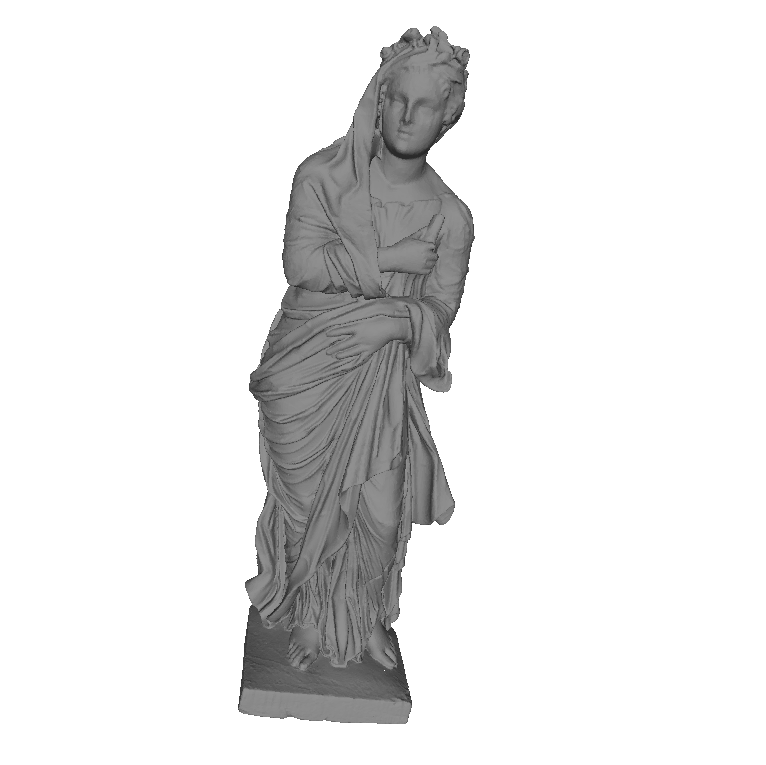
\includegraphics[width=\linewidth]{./Figures/train-dataset/41.vestalin.png}
		\caption{Vestalin}
	\end{subfigure}
	\begin{subfigure}[b]{0.23\linewidth}
		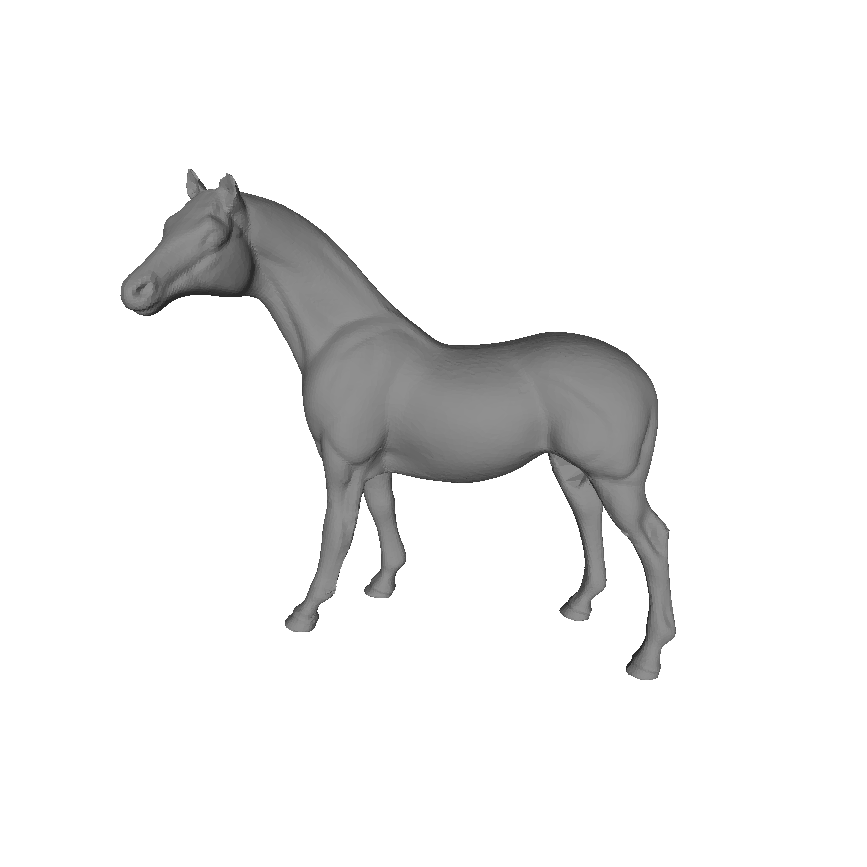
\includegraphics[width=\linewidth]{./Figures/train-dataset/42.zebra.png}
		\caption{Zebra}
	\end{subfigure}
	\begin{subfigure}[b]{0.23\linewidth}
		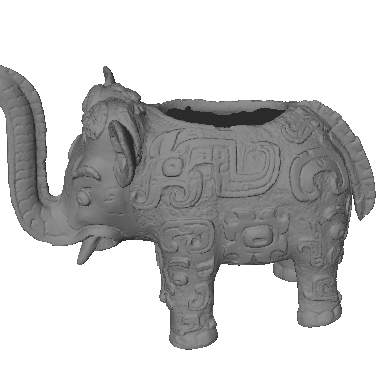
\includegraphics[width=\linewidth]{./Figures/train-dataset/43.elephant-zun-base.png}
		\caption{elephant-zun-base}
	\end{subfigure}

	\begin{subfigure}[b]{0.23\linewidth}
		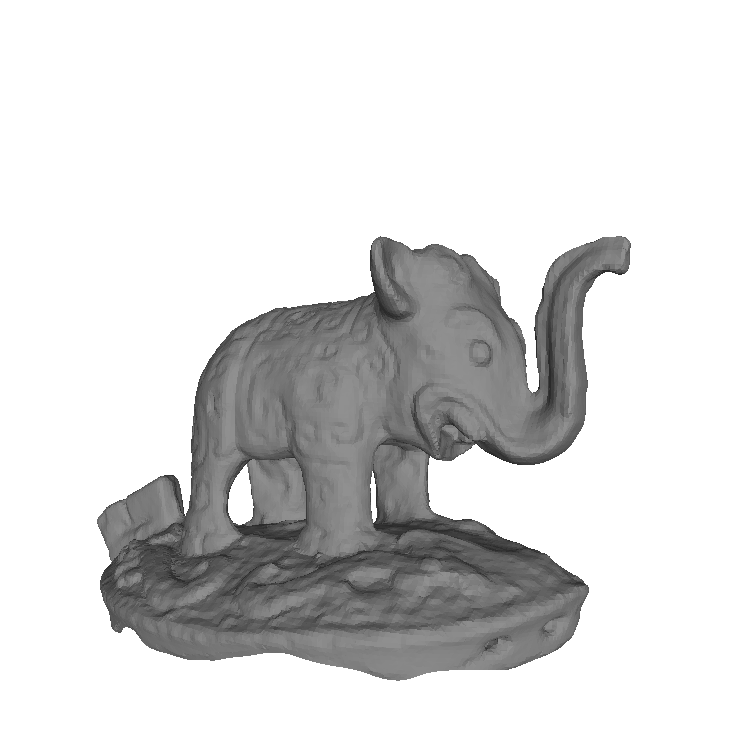
\includegraphics[width=\linewidth]{./Figures/train-dataset/44.elephant-zun-lid.png}
		\caption{elephant-zun-lid}
	\end{subfigure}
	\begin{subfigure}[b]{0.23\linewidth}
		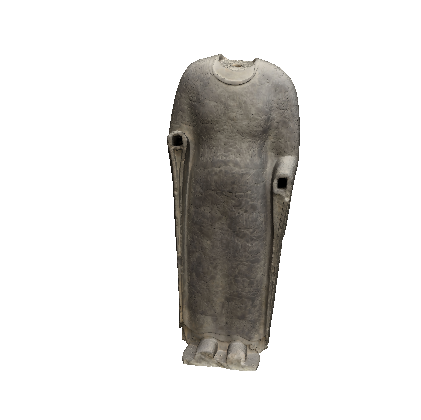
\includegraphics[width=\linewidth]{./Figures/train-dataset/45.cosmic-buddha.png}
		\caption{cosmic-budda}
	\end{subfigure}
	\begin{subfigure}[b]{0.23\linewidth}
		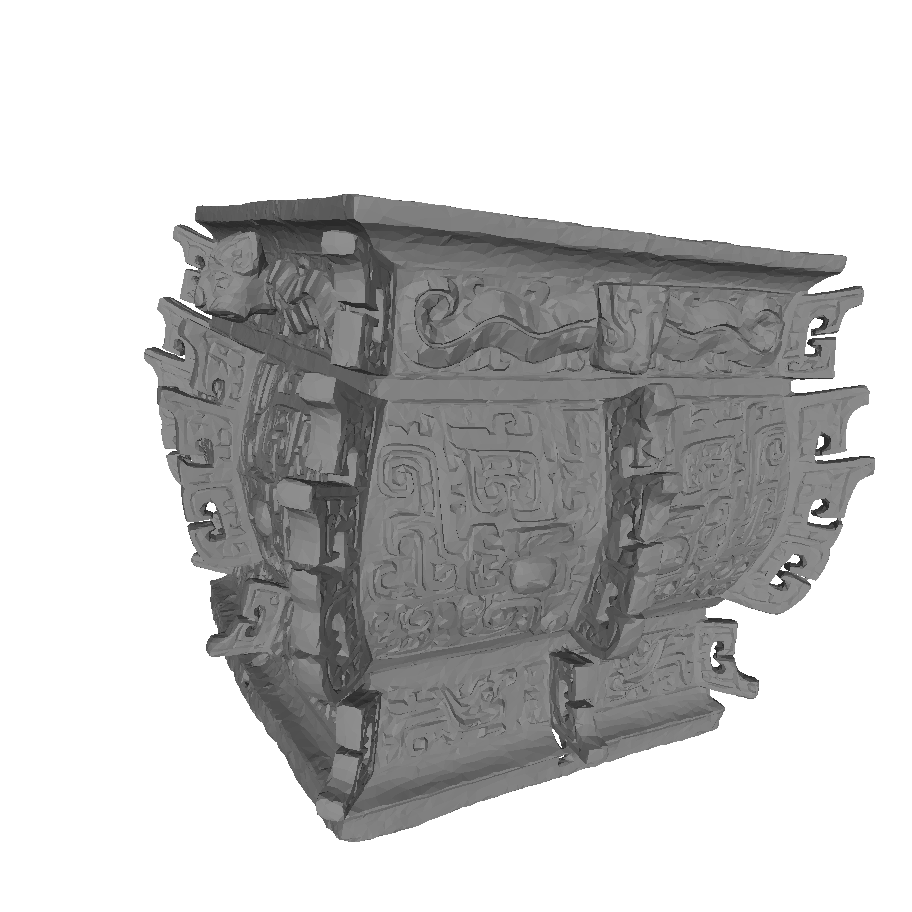
\includegraphics[width=\linewidth]{./Figures/train-dataset/46.fangyi-base.png}
		\caption{fangyi-base}
	\end{subfigure}
	\begin{subfigure}[b]{0.23\linewidth}
		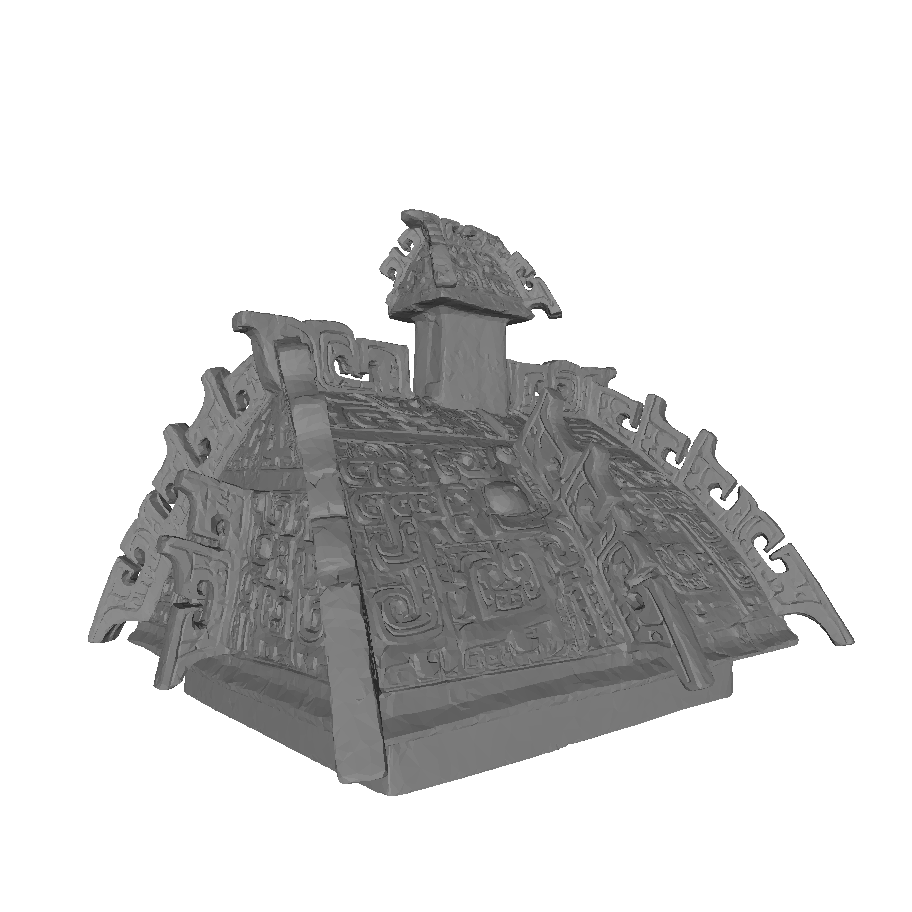
\includegraphics[width=\linewidth]{./Figures/train-dataset/47.fangyi-lid.png}
		\caption{fangyi-lid}
	\end{subfigure}

	\begin{subfigure}[b]{0.23\linewidth}
	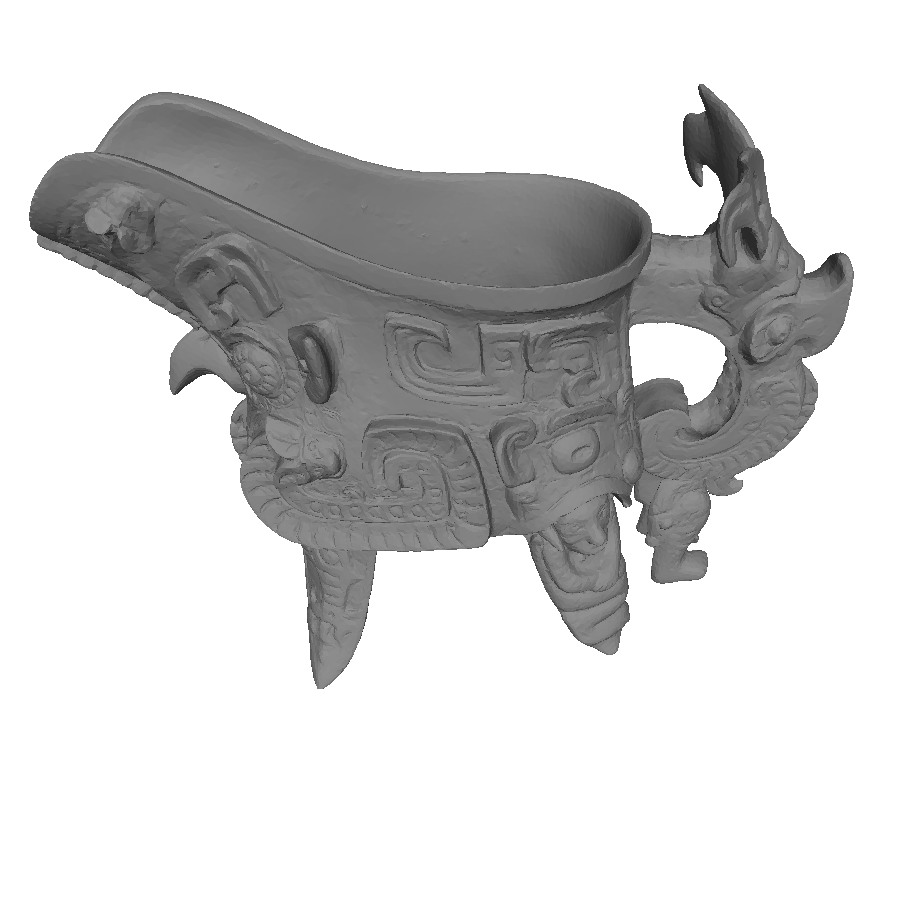
\includegraphics[width=\linewidth]{./Figures/train-dataset/48.guang-base.png}
	\caption{guang-base}
\end{subfigure}
\begin{subfigure}[b]{0.23\linewidth}
	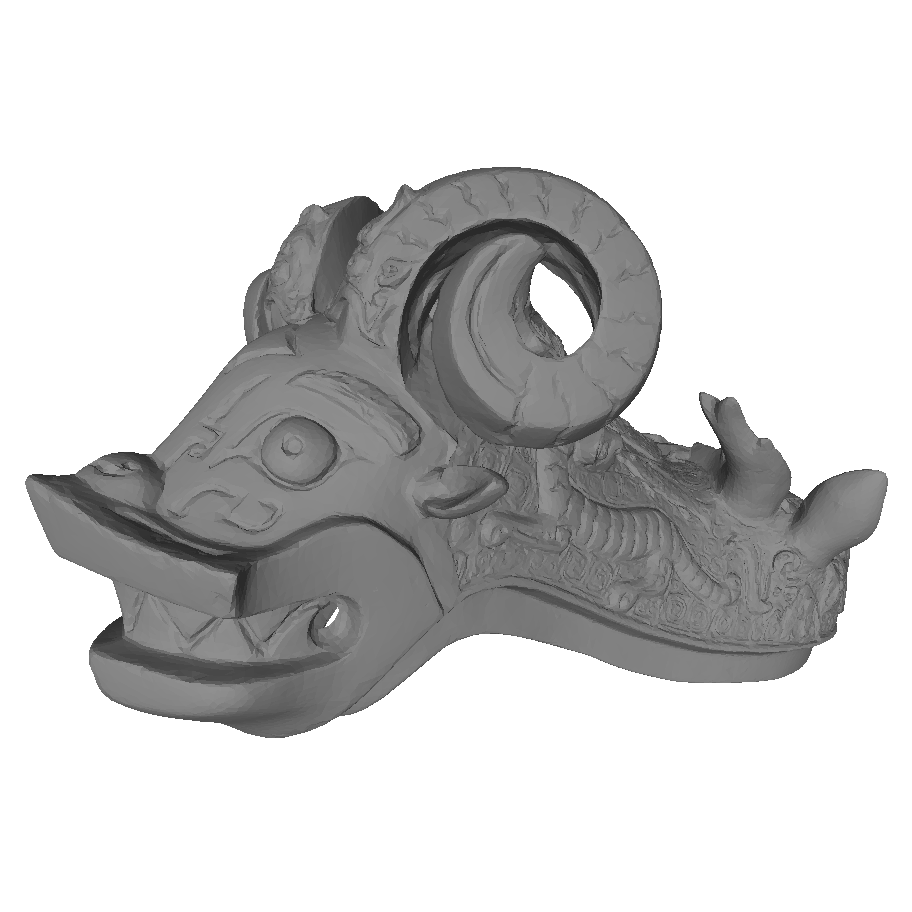
\includegraphics[width=\linewidth]{./Figures/train-dataset/49.guang-lid.png}
	\caption{guang-lid}
\end{subfigure}
\begin{subfigure}[b]{0.23\linewidth}
	\includegraphics[width=\linewidth]{./Figures/test-dataset/00.garfield.png}
	\caption{Garfield}
\end{subfigure}
\begin{subfigure}[b]{0.23\linewidth}
	\includegraphics[width=\linewidth]{./Figures/test-dataset/01.Bus.png}
	\caption{bus}
\end{subfigure}

\begin{subfigure}[b]{0.23\linewidth}
	\includegraphics[width=\linewidth]{./Figures/test-dataset/02.dragon.png}
	\caption{dragon}
\end{subfigure}
\begin{subfigure}[b]{0.23\linewidth}
	\includegraphics[width=\linewidth]{./Figures/test-dataset/03.baoshanlu.png}
	\caption{baoshanlu}
\end{subfigure}
\begin{subfigure}[b]{0.23\linewidth}
	\includegraphics[width=\linewidth]{./Figures/test-dataset/04.washington.png}
	\caption{Washington}
\end{subfigure}
	
	\label{fig:dataset_c}
	\caption{Point clouds in training dataset C}
\end{figure}
